\documentclass[10pt,twocolumn,letterpaper]{article}
\usepackage[T1]{fontenc}
\usepackage[pagenumbers]{cvpr}
\usepackage{amsmath,amssymb,amsthm,booktabs,graphicx,microtype,array}
\definecolor{cvprblue}{rgb}{0.21,0.49,0.74}
\usepackage[breaklinks,colorlinks,allcolors=cvprblue]{hyperref}
\newtheorem{proposition}{Proposition}
\newcommand{\R}{\mathbb R}\newcommand{\E}{\mathbb E}
\newcommand{\norm}[1]{\left\lVert#1\right\rVert}
\title{LatentAtlas: Few-Anchor Interfaces for Frozen Reward Transfer Across Autoencoders\\Supplementary Material}
\author{Anonymous authors}
\begin{document}\maketitle
\setcounter{section}{0}\renewcommand{\thesection}{\Alph{section}}

\section{Guide to the Evidence}
This supplement specifies the clean-image adaptation protocol, fitted interfaces, statistical definitions, and mathematical interpretation of the main paper. Its experiments use three distinct target contracts. The FLUX and Cosmos comparisons map directly to the reference encoding of the original image ($T_0$). The DC-AE localization compares that direct mapping to a decode--re-encode route ($T_1$). The DC-AE fitting-support study trains toward $T_1$ and measures agreement with its frozen reward $G$. Table~\ref{tab:datasets} keeps their sample identities and evaluation targets separate.

\begin{table*}[t]\centering\small
\resizebox{\textwidth}{!}{\begin{tabular}{lllll}
\toprule
Study & Fitting/validation images & Evaluation & Training target & Agreement target\\
\midrule
FLUX/Cosmos direct transfer &64 / 64&28 groups, 252 images, 1,008 pairs&$T_0$&native $T_0$ reward\\
Cosmos ridge/A1/A2 &64 / 64&same 28 groups and pairs&$T_0$&native $T_0$ reward\\
DC-AE direct/round-trip &64 / 64 for direct&same 28 groups and pairs&$T_0$ for direct&native $T_0$ reward\\
DC-AE small/Strong &64 / 64&same 28 groups and pairs&$T_1$&native $T_0$ reward\\
DC-AE support expansion &64 or 256 / 64&56 groups, 504 images, 2,016 pairs&$T_1$&$G$, reward on $T_1$\\
\bottomrule
\end{tabular}}
\caption{Experiment identities. Each physical pair has four fixed scoring streams. The 56 groups are disjoint from the 28 adapter development groups; their parent pool had already been used for source qualification.}
\label{tab:datasets}\end{table*}

\section{Encoding and Frozen Scoring}
\subsection{Model Identity}
The reference is SD3.5-Medium, and the reward is DiNa's 12-layer SD3.5M model~\cite{liu2026beyond}. Table~\ref{tab:models} specifies the exact public model identifiers and abbreviated revision hashes. Cosmos is a continuous image autoencoder. The FLUX and Cosmos source representations have 16 channels and an eightfold spatial reduction; DC-AE has 32 channels and a 32-fold reduction.

\begin{table*}[t]\centering\small
\begin{tabular}{ll}
\toprule
Model repository / component & Revision (first 12 hexadecimal digits)\\
\midrule
\texttt{stabilityai/stable-diffusion-3.5-medium} (VAE) &\texttt{b940f670f0ed}\\
\texttt{liuhuohuo/DiNa-LRM-SD35M-12layers} &\texttt{31d99dc51bf4}\\
\texttt{black-forest-labs/FLUX.1-schnell} (VAE) &\texttt{741f7c3ce8b3}\\
\texttt{nvidia/Cosmos-0.1-Tokenizer-CI8x8} &\texttt{04792f8b318a}\\
Cosmos official tokenizer code &\texttt{3584ae752ce8}\\
\texttt{mit-han-lab/dc-ae-f32c32-in-1.0-diffusers} &\texttt{ebe8371e61a7}\\
\bottomrule
\end{tabular}
\caption{Frozen encoder and reward identities. Full hashes and weight checksums accompany the source manifests.}
\label{tab:models}\end{table*}

DiNa uses its 12-layer SD3.5M readout, visual/text features at layers 4/8/12, four queries, and its active LoRA adapter. All parameters are in evaluation mode with gradients disabled during scoring. Freezing preserves the learned adapter's contribution; disabling it would change the reward being evaluated.

\subsection{RGB Geometry and Latent Coordinates}
An image is identified by its original byte SHA256. PIL converts it to RGB. For original size $(W,H)$, define $D=\max(1024,W,H)$ and transform each side $s\in\{W,H\}$ to
\begin{equation}
 s'=\max\!\left(16,16\left\lfloor\frac{\lfloor1024s/D\rfloor}{16}\right\rfloor\right).
\end{equation}
The image is resized by Lanczos, without a center crop or EXIF transpose. This keeps large images within 1,024 pixels on the long side, preserves variable aspect ratios up to rounding, and avoids enlarging ordinary smaller images. SD3.5, FLUX, and Cosmos receive the same effective RGB geometry. Their tensors have shape $[1,16,H'/8,W'/8]$.

SD3.5 and FLUX pixels are converted in FP32 as $(u/255-0.5)/0.5$, rearranged to NCHW, then cast to BF16 for the model. Cosmos uses its official tensor conversion from the same RGB array to the $[-1,1]$ range. The reference VAE takes a seeded posterior sample and applies
\begin{equation}
 z_r=(q_r-0.0609)\,1.5305.
\end{equation}
FLUX supplies the raw posterior mode, without generator-pipeline scaling, shift, or packing. Cosmos supplies its raw continuous tensor, without a KL-posterior draw. REC and A2 learn the normalized reference target directly; their outputs receive no second application of the shift/scale.

For reproducible reference encoding, the posterior seed is a deterministic hash of the namespace \texttt{DINA\_SRC0\_HPDV3\_}\allowbreak\texttt{SOURCE\_DOMAIN\_PARITY\_R1}, the tag \texttt{native\_sd35\_latent}, and the image byte identity. Canonical compact UTF-8 JSON is SHA256-hashed; the first eight bytes, interpreted big-endian, are reduced modulo $2^{63}$. A CUDA generator on the input device supplies the posterior draw. Historical projector training uses initialization and sampling seed 20260827; the matched comparison uses 2026101901. All subsequent comparisons bind the cached encodings by hash, including the first validated Cosmos cache where cross-process bitwise equality was not guaranteed.

\subsection{Reward Calls and Noise Coupling}
The clean reference or mapped tensor enters
\begin{equation}
 D_\phi((1-\sigma_\tau)z+\sigma_\tau\xi,c,t_\tau),
\end{equation}
with $\sigma_\tau=0.4002932608127594$ and $t_\tau=400.29327392578125$. Prompt processing and the active reward weights are fixed. Four stored noise streams evaluate each physical pair. Native and mapped arms share the appropriate candidate-occurrence noise stream. The same image appearing in another comparison can have a different occurrence-level noise identity, so the records are analyzed as paired occurrences with group dependence. Reconstructing one universal image score from those repeated rows would change the experiment.


\section{Historical Projectors and Controls}
\label{sec:historical}
Tables~\ref{tab:architectures} and~\ref{tab:main} retain the historical fitting procedures and results used for correspondence controls and functional diagnostics. Their optimization budgets differ from the matched strong-baseline comparison in Section~\ref{sec:matched-protocol}.

\begin{table}[t]
\centering\small
\begin{tabular}{lrrr}
\toprule
Interface & Parameters & Field & Selected step\\
\midrule
Pointwise ridge &272&$1\times1$&closed form\\
Spatial ridge &6,416&$5\times5$&closed form\\
A1 (pointwise MLP)&2,128&$1\times1$&360\\
REC (SiLU)&39,056&$3\times3$&1,000\\
A2 (GELU)&40,216&$3\times3$&2,500\\
\bottomrule
\end{tabular}
\caption{Historical Cosmos interfaces, each using the same 64 FIT and 64 VAL images. A1 uses batch 8; REC and A2 use batch 32. Selected steps exclude additional search runs.}
\label{tab:architectures}
\end{table}

\begin{table*}[t]
\centering\small
\begin{tabular}{llrrrr}
\toprule
Source & Interface & Parameters & Native agreement (\%)$\uparrow$ & Margin MSE$\downarrow$ & Human accuracy (\%)$\uparrow$\\
\midrule
SD3.5 & Native &--&100.00&0&72.82\\
FLUX & REC &39,056&91.69&0.4315&72.79\\
Cosmos & Untrained REC &39,056&59.68&--&44.62\\
Cosmos & Permuted-pair REC &39,056&59.43&--&49.08\\
Cosmos & Pointwise ridge &272&90.91&0.4604&72.02\\
Cosmos & Spatial ridge $5\times5$ &6,416&89.33&0.5139&71.70\\
Cosmos & A1 &2,128&92.15&0.3466&72.30\\
Cosmos & REC &39,056&93.41&0.2338&72.62\\
Cosmos & A2 &40,216&94.75&0.1584&72.62\\
\bottomrule
\end{tabular}
\caption{Historical clean transfer to the original SD3.5 reference, on the same development groups. All fitted interfaces use 64 FIT and 64 VAL images. Native agreement evaluates the reward's existing decisions; human accuracy evaluates annotated preferences. REC/A2 have different update and search budgets (Table~\ref{tab:architectures}). Dashes indicate an unreported endpoint, not a zero.}
\label{tab:main}
\end{table*}
\subsection{REC and Controls}
For 16-channel sources, REC is
\begin{equation}
 P(q)=C_{1,64\to16}\big[\operatorname{SiLU}(C_{3,64\to64}[\operatorname{SiLU}(C_{1,16\to64}(q))])\big].
\end{equation}
Here $C_{k,a\to b}$ is a convolution with kernel size $k$, bias, stride one, and spatially preserving padding. The parameter count is
$(16\cdot64+64)+(9\cdot64^2+64)+(64\cdot16+16)=39,056$.
The DC-AE direct variant changes the input width to 32, giving 40,080 parameters, and applies the recorded grid conversion.

AdamW uses learning rate $3\times10^{-4}$, betas $(0.9,0.95)$, epsilon $10^{-8}$, weight decay $10^{-4}$, \texttt{foreach=False}, and gradient norm clipping at one. Effective batch 32 is implemented through 32 single-image microbatches, accommodating variable grids. Parameters are FP32, CUDA forward computation uses BF16 autocast, and the saved output contract is BF16. The schedule retains the first 1,000 steps of the original 12,000-step cosine schedule, including 500 warm-up steps and the original $3\times10^{-5}$ floor. It is not a cosine schedule compressed to 1,000 steps.

The fitting objective is the image-balanced, FIT-channel-variance-weighted MSE in the main paper. Validation at steps 500 and 1,000 selects the correct-pair checkpoint at 1,000. The permuted control selects 500 using true validation correspondence. The untrained control uses the dimension-compatible initialized adapter. The controls establish effects of the recorded fitting procedure and fitting correspondence, with one permutation and initialization.

\subsection{A1: Adapted Local Feature Matching}
A1 applies a shared per-position linear map $16\to64$, ReLU, and a linear map $64\to16$, totaling 2,128 parameters. It adapts the local-feature-matching operator of foundation-model stitching~\cite{mai2026revisiting} to the present coordinate interface. Its actual objective is unweighted coordinate MSE, with image-balanced averaging. It uses no final reward features or task loss.

AdamW uses betas $(0.9,0.999)$, epsilon $10^{-8}$, weight decay $0.01$, and gradient clipping at one. Constant learning rates $0.001$, $0.005$, and $0.01$ are compared, with batch eight, a maximum of 800 updates, validation every eight updates, and early stopping after at least 40 updates when five consecutive validation checks fail to improve the strict minimum (relative minimum gain zero). The lowest-VAL model is selected; ties prefer the lower learning rate and earlier step. The selected model is learning rate $0.005$ at step 360. Intermediate computation is FP32 and outputs follow the BF16 scoring contract. This is an operator adaptation, with the objective and selection procedure stated here.

\subsection{A2: Spatial GELU Mapping}
A2 is a $3\times3$ convolution $16\to144$, exact GELU, a $1\times1$ convolution $144\to120$, exact GELU, and a $1\times1$ output $120\to16$. Every convolution has a bias. The parameter count is 40,216, 2.97\% above REC. Its spatial receptive field is $3\times3$.

A2 uses REC's weighted coordinate objective, batch size 32, AdamW hyperparameters, gradient clipping, and precision contract. Learning rates $10^{-4}$, $3\times10^{-4}$, and $10^{-3}$ are each trained to 1,000 steps and continued to 2,500 without resetting optimizer, sampler, RNG, or the original 12,000-step schedule. The selected checkpoint uses $10^{-3}$ at step 2,500. This endpoint is the first common cohort satisfying the convergence, stability, and precision criteria below for all three rates. One final A2 checkpoint is evaluated in the reported comparison, with the full search history counted as development.

At a common horizon $h$ (1,500, 2,000, 2,500, and so on), let $v_1,\ldots,v_6$ be the six validation NMSEs at $h-250,h-200,\ldots,h$. Qualification requires the median decrease from the first three to the last three, divided by the first median, to be at most 1\%; the range of all six divided by their median to be at most 2\%; and the median prediction-change NMSE of the last three adjacent 50-step pairs, divided by selected VAL NMSE, to be at most 5\%. Denominators are floored at $10^{-12}$. Selected VAL NMSE must also be at most $1.25\times0.10731854173354805$, the REC reference. For every validation image, deployed-versus-FP32-shadow NMSE divided by shadow-to-target NMSE (floored at $10^{-6}$) must be at most $0.001$.

Eligible checkpoints are the original steps 500/1,000 and common 500-step continuation horizons. Each run retains the strict VAL minimum, keeping the earlier step on a tie. Across rates, selection sorts by VAL loss, learning rate, then step. The 50-step diagnostics assess qualification; they are not additional eligible selected checkpoints.

REC processes 32,000 fitting-image presentations for its selected run, whereas each complete A2 run processes 80,000. A1 differs in parameter count, receptive field, objective weighting, and optimizer settings. These are comparisons of fitted procedures, with those differences preserved.

\subsection{Shared Ridge Baselines}
Let $u$ denote a source feature vector at one location, or the concatenation of its $5\times5$ neighborhood. FIT-only source mean and standard deviation define standardized features. The fitted affine map solves the centered normal equations
\begin{equation}
 (C_{uu}+\lambda I)W=C_{uz},
\end{equation}
with an unpenalized intercept. Sufficient statistics give equal total weight to each image. Pointwise fitting compares $\lambda\in\{0,0.001\}$ on VAL64 and selects $0.001$. Its input dimension is 16 and its parameter count is $16(16+1)=272$. A standard deviation below $10^{-12}$ is replaced by one in that implementation.

Spatial ridge uses 400 features, 16 outputs, and 6,416 parameters. A source variance floor of $10^{-6}$ is used; each channel's normalization is shared across its 25 offsets. The selected radius is two ($5\times5$), preferred on coordinate validation over the evaluated $3\times3$ alternative, with $\lambda=0.001$. Fitting and the principal coordinate diagnostic use the common four-pixel border crop. Full-grid reward evaluation uses the predeclared reflect-padding implementation.

Coefficients are fitted in FP64 and absorb the FIT normalization into the stored weight and bias. Deployment applies the affine map to raw source coordinates with FP32 matrix multiplication, TF32 disabled, then casts to BF16. Applying source normalization a second time would change the evaluated baseline. Coordinate values reported for these baselines come from their archived CPU-BF16 diagnostic; the actual reward results come from complete DiNa evaluations.

\section{Matched Cosmos and FLUX Comparisons}
\label{sec:matched-protocol}
\paragraph{Data and information.}
The five methods use the original 64 FIT and 64 VAL images, with identical cached source and reference tensors. All parameter updates and checkpoint choices use coordinates only. Both sources evaluate the same original 252 images in 28 development groups, four occurrence-level noise streams, and native-score cache. The FLUX source manifest replaces only source-coordinate bindings; reference targets, image identities, prompts, pair orientation, and noise seeds remain unchanged. No reward calls inform training or checkpoint selection.

\paragraph{Optimization and selection.}
Each of REC, A2, Interposer-MSE, and Interposer-cycle receives learning rates $\{10^{-4},3\times10^{-4},5\times10^{-4},10^{-3}\}$, 2,500 updates per rate, effective batch 32, seed 2026101901, and validation every 125 updates. REC, A2, and Interposer-MSE use the image-balanced variance-weighted objective and REC optimizer/schedule specified above. Each family's best BF16 VAL NMSE over updates 2,125--2,500 is compared with its best over updates 125--2,000. A relative improvement of at least 1\% triggers a common extension. Cosmos cycle triggers this rule at 3.36\%; FLUX A2 and cycle trigger at 1.35\% and 1.75\%. Each source therefore gives all four families a continuation at their own coordinate-selected rate, from the complete step-2,500 state to step 5,000. Each receives 20 additional validation points, for 100 candidates per family. Minimum VAL NMSE selects the checkpoint, with ties preferring earlier updates, then lower rates. The corresponding final comparison of the last 500 updates against earlier candidates triggers no further extension; this is a stopping rule, not a proof of optimization convergence.

\begin{table}[t]\centering\small
\begin{tabular}{lrrr}
\toprule
Family & Rate & Step & VAL NMSE\\
\midrule
\multicolumn{4}{l}{\textit{Cosmos source}}\\
REC &.001&5,000&.094591\\
A2 &.001&5,000&.093156\\
Interposer-MSE &.001&4,500&.128712\\
Interposer-cycle &.0005&4,750&.133508\\
Spatial affine &$\lambda=0$&closed form&.119379\\
\midrule
\multicolumn{4}{l}{\textit{FLUX source}}\\
REC &.001&5,000&.140261\\
A2 &.001&5,000&.132502\\
Interposer-MSE &.001&4,500&.203361\\
Interposer-cycle &.0003&5,000&.213491\\
Spatial affine &$\lambda=.001$&closed form&.150377\\
\bottomrule
\end{tabular}
\caption{Source-specific selections fixed before reward evaluation. Both affine choices use a $5\times5$ neighborhood.}
\end{table}

\paragraph{Strong affine baseline.}
We fit all combinations of neighborhood size $k\in\{1,3,5\}$ and ridge strength $\lambda\in\{0,10^{-4},10^{-3},10^{-2},10^{-1}\}$. Full-image reflect-padded neighborhoods are shared between fitting and deployment. FIT-only feature standardization, an unpenalized intercept, image-balanced FP64 sufficient statistics, and the same FIT teacher variance define the fit. The zero-ridge solver uses a relative eigenvalue cutoff of $10^{-12}$. Validation evaluates the deployed FP32-to-BF16 prediction. Each selected $5\times5$ map has 6,416 parameters; fitting and selection use CPU only.

\paragraph{Interposer adaptations.}
We use SD-Latent-Interposer commit \texttt{9344ddf53c3f} and its 1,432,720-parameter forward architecture~\cite{city96latentinterposer}. The MSE variant shares REC's loss and optimization. The cycle variant retains the released \texttt{fx-to-v3} objective weights $p=1,r=.1,b=1,h=0$. A forward map $F$ minimizes $\|F(q)-z\|_1+.1\|B(F(q))-q\|_1$; a separate reverse map $B$ minimizes $\|B(z)-q\|_1$. Gradients through both networks are computed for the first loss, and its reverse-network gradients are cleared before the independent reverse update. Both use AdamW with betas $(.5,.95)$, weight decay .01, constant learning rate, and no gradient clipping. Reverse initialization uses seed 2026101902. Full-image microbatch one accumulated to 32 gives per-image spatial BatchNorm statistics; the released batch size is 48. BF16 replaces the released FP16 autocast, and the present finite data and update budgets replace its original training setting. The deployed interface is the forward map only.

\paragraph{Computation.}
Per source, 16 initial runs and four continuations use 2,400,000 image-level network forwards and corresponding network backward traversals, 62,500 optimizer updates, and 25,600 validation forwards. Supervised single-GPU time is 15.144 hours for Cosmos and 14.900 hours for FLUX. A cycle update processes three network forwards and two optimizer steps per batch; equal opportunities therefore entail different FLOPs. Each source makes 40,320 scientific single-image DiNa calls and 104 technical checks. Cosmos generates 24 prompt caches with 72 text-encoder calls and reuses four; FLUX reuses all 28 exact caches, adding zero text calls. Scoring lasts 5,710.411 and 5,677.120 seconds, respectively. Each source requires 1,270 interface predictions: 1,016 neural and 254 affine, including qualification inputs. FLUX requires 256 source-VAE encodings (252 evaluation images and four parity checks), taking 233.519 seconds; Cosmos reuses its source cache. No generator is invoked. Training, selection, and evaluation costs have separate ledgers.

\paragraph{Uncertainty and verification.}
We use 50,000 PCG64 bootstrap draws with seed 2026101902, resampling the 28 lexicographically ordered groups and retaining all their pair-streams. The same draws serve every method. For each source separately, ten method pairs and two primary endpoints form the predeclared 20-comparison family; central percentile intervals use quantiles .00125 and .99875. Absolute margin-MSE differences carry inference; relative reductions are descriptive. Human accuracy and native regret use ordinary descriptive 95\% intervals. All 40,320 scientific score records in each source join to the original image, prompt, seed, input-tensor, and actual-call identities. An independent implementation reproduces the group sufficient statistics and all reported estimates and intervals. These intervals are conditional on fixed checkpoints and the development sample; they exclude uncertainty from resampling the Anchor bank or repeating selection. Shared images and native scores couple the two source comparisons; we report each source separately without treating them as independent samples or a joint 95\% family.

\section{DC-AE Targets, Capacity, and Coverage}
\subsection{Source and Teacher Geometry}
DC-AE encoding uses raw, unscaled FP32 latents with 32 channels and spatial shape $\lfloor H'/32\rfloor\times\lfloor W'/32\rfloor$. Its official tiled implementation uses a 512-pixel tile and 448-pixel step. The image input remains the variable-size RGB geometry above; tile sizes do not specify a center crop.

For a bridge, the raw source is bilinearly resized to the explicit reference target grid, with \texttt{align\_corners=False}. For the round-trip teacher, the source decoder first reconstructs RGB. Decoder output is converted from $[-1,1]$ to FP32 $[0,1]$ and clamped. The bridge removes recorded padding, restores the effective RGB dimensions with bilinear interpolation when needed, and converts to the reference encoder's input range. The current teacher construction uses zero explicit padding; 96 of the original 252 evaluation images required size restoration. The reference encoder takes the fixed-seed posterior sample and applies the usual reference scale and shift. Thus $T_1$ includes the actual reconstruction and resizing path.

The original reference $T_0$ encodes the input RGB directly. Its reward $N$ and the reward $G$ on $T_1$ are both produced by the same frozen DiNa. Students trained toward $T_1$ can be evaluated against $G$, against $N$, and against human labels; each endpoint retains that name.

\subsection{Strong Architecture}
Strong first resizes the 32-channel source grid, then applies a biased $1\times1$ stem $32\to64$ with SiLU. It contains 12 residual blocks
\begin{equation}
 h\longmapsto h+C_3\big(\operatorname{SiLU}(C_3(h))\big),
\end{equation}
where both convolutions have 64 input/output channels, kernel three, stride one, zero padding one, and bias. There is no activation after residual addition. A linear biased $1\times1$ tail maps $64\to16$. There is no normalization layer or dropout. The count is $2,112+12(73,856)+1,040=889,424$ parameters.

The small bridge uses the 32--64--64--16 REC architecture with 40,080 parameters. The small/Strong comparison uses 2,000 updates, batch 32, the original 12,000-step learning-rate schedule, and $T_1$ targets. On the 28-group development set, the small bridge has mean $T_1$ coordinate NMSE 0.309153733 and Strong has 0.310404429. The relative reduction is $-0.405\%$, with a 95\% interval $[-2.732,1.994]\%$. Strong's human and original-reference ($T_0$) agreement gains have adjusted lower bounds of 1.54 and 3.50 pp, respectively. The coordinate interval is unresolved; it is not an equivalence test.

\subsection{FIT64 versus FIT256}
The support expansion retains Strong, $T_1$, initialization seed 20260827, batch 32, and 2,000 updates. FIT256 consists of the original 64 images and 192 additional images from the same COCO pool. VAL64 is fixed, so total paired-image exposure is 128 or 320. Both arms train from the original step-zero state.

A seeded permutation sampler visits the support in successive randomized epochs. In the fixed 64,000-image draw sequence, FIT64 images occur 1,000 times each and FIT256 images 250 times each. Each optimizer update accumulates 32 single-image gradients. Training preserves the original AdamW and learning-rate schedule. The normalized loss uses the original FIT64 $T_0$ channel-variance weights, denoted $W_0$, in both arms; the teacher tensors themselves are $T_1$. Keeping $W_0$ fixed makes the loss weighting identical across the support comparison.

The 56-group evaluation contains 504 images and 2,016 pairs. Its group identities are disjoint from the earlier adapter development groups, while its parent 400-group pool had source-qualification exposure. Original endpoint intervals use 20,000 paired group-bootstrap draws and three-endpoint-adjusted quantiles $1/120$ and $119/120$.

\section{Metrics and Statistical Interpretation}
\subsection{Definitions and Ties}
Let $m_{p,k}^{M}=s_{a,p,k}^{M}-s_{b,p,k}^{M}$ be the margin for method $M$ on pair $p$ and stream $k$. Let $y_p\in\{-1,+1\}$ encode the human-preferred orientation. Human accuracy is
\begin{equation}
 \operatorname{Acc}(M)=\frac1{PK}\sum_{p,k}\mathbf1\{y_pm_{p,k}^{M}>0\}.
\end{equation}
Ties receive zero credit. For native method $N$, let $V=\{(p,k):m_{p,k}^N\ne0\}$. Native agreement is
\begin{align}
 a_{p,k}&=\mathbf1\{m^M_{p,k}m^N_{p,k}>0\}+\tfrac12\mathbf1\{m^M_{p,k}=0\},\\
 \operatorname{Agr}(M,N)&=\frac1{|V|}\sum_{(p,k)\in V}a_{p,k}.
\end{align}
Margin MSE includes every pair-stream:
\begin{equation}
 \operatorname{MMSE}(M,N)=\frac1{PK}\sum_{p,k}(m^M_{p,k}-m^N_{p,k})^2.
\end{equation}
These definitions explain why agreement and human accuracy can differ even for the same interface. For the direct main comparison, $PK=4,032$ and $|V|=3,999$. Agreement with $G$ uses $G$'s own non-tie mask.

For Native regret, a mapped tie uses the expected native score under a uniform choice. The pair-stream loss is
\begin{equation}
 \ell_{p,k}^{M}=|m_{p,k}^{N}|\!\left[\mathbf1\{m_{p,k}^{M}m_{p,k}^{N}<0\}
 +\tfrac12\mathbf1\{m_{p,k}^{M}=0\}\right].
\end{equation}
Native ties contribute zero. We average $\ell_{p,k}^{M}$ over all $PK$ pair-streams. Selection is performed separately within each stream; averaging scores before choosing would define a different endpoint. Scores retain their candidate-occurrence noise identities, so these pairwise records are not pooled into one shared nine-candidate score vector. This complementary descriptive endpoint preserves the primary agreement and margin-MSE analysis families.

Coordinate NMSE averages the weighted spatial error within each image, then equally across images. A shared spatial model receives many correlated locations from one image; an image count remains an image count. The coordinate norm used in the mathematical bounds is an explicitly chosen Euclidean norm, not automatically this variance-weighted reporting metric.

\subsection{Resampling and Analysis Families}
Pairwise outcomes sharing images or prompts are dependent. The archived analyses resample the connected groups as clusters, keeping all pair/stream contributions within a selected group. Intervals are conditional on the fixed evaluated checkpoints. Development choices made before these comparisons remain part of the data's history.

The ridge analysis uses its original nine-endpoint simultaneous family. The A1/A2 analysis uses six effects and saved quantiles $0.0020833333$ and $0.9979166667$. For REC minus A2, the agreement interval is $[-3.202407,0.012513]$ pp and the human interval is $[-2.058532,1.959325]$ pp. The normalized MSE effect is $(\operatorname{MMSE}(B,N)-\operatorname{MMSE}(A,N))/(\operatorname{MMSE}(B,N)+\operatorname{MMSE}(A,N))$, set to zero when both errors vanish. For $A=$REC and $B=$A2, its interval is $[-0.302202,-0.064927]$, with the effect oriented so negative values favor REC's comparator A2. The main paper reports the direct relative reduction in raw margin MSE separately. These conditional bootstrap intervals do not correct for all historical scientific consumption.

Cosmos REC also had a historical registered tolerance check: the central 90\% interval for human accuracy relative to native was $[-1.513,1.042]$ pp, above the allowed $-2$ pp lower boundary, and the agreement lower bound was 91.662\%, above 90\%. This establishes that historical tolerance check on its development data. FLUX did not pass the same recorded gate, so closeness of the human point estimates is not used to label all sources equivalent.

\subsection{Historical Joint Decision Decomposition}
\begin{figure}[t]
\centering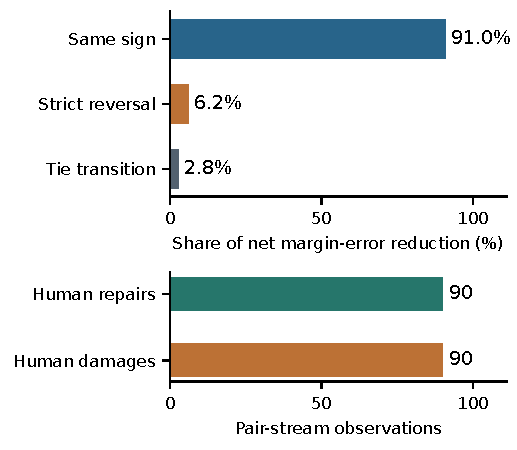
\includegraphics[width=\columnwidth]{figures/clean/endpoints.pdf}
\caption{Historical Cosmos REC-to-A2 joint analysis. The net reduction in summed squared margin error is partitioned by ternary decision transition. Signed contributions are aggregated within each partition. Human-preference repairs and damages balance at 90 each across 4,032 pair-stream observations.}
\label{fig:joint}
\end{figure}
For REC and A2 define a per-row signed improvement
\begin{equation}
 g_{p,k}=(m^{\rm REC}_{p,k}-m^N_{p,k})^2-(m^{\rm A2}_{p,k}-m^N_{p,k})^2.
\end{equation}
Partition rows by whether their ternary signs are equal, strictly reversed, or transition to/from a tie. Summing $g$ over these disjoint sets exactly partitions the total net MSE gain. The three counts are 3,821, 142, and 69. Their signed gain fractions are 0.9099909, 0.0619909, and 0.0280182 (rounding accounts for the last digit). In the unchanged-sign set, 1,475 rows have negative individual gain. The aggregate fraction therefore describes where the net gain occurs, not the fraction of improved examples.

A human repair changes an incorrect or tied prediction into a correct one; a damage changes a correct one into an incorrect or tied prediction. Across all rows there are 90 of each. Native strict repairs and damages are 89 and 47, and the total half-credit native gain is 53.5. Human and native correctness are different reference labels. The decomposition is an exact retrospective description of these stored outcomes, not an independent validation sample or a mechanistic causal intervention.

\section{Elementary Functional Conditions}
The following derivations formalize the interpretation used in the paper. They build on standard linear identifiability and readout-stability arguments~\cite{csiszarik2021similarity,insulla2025alignment}. Their role is to state precisely what coordinate supervision does and does not determine in a specified model class.

\subsection{Pairwise Stability}
\begin{proposition}
For fixed candidate prompts and coupled native/mapped noise, define $e_a,e_b$ as mapped-minus-native score errors. Then $\widehat\Delta=\Delta+e_a-e_b$. If $\Delta\ne0$ and $|e_a-e_b|<|\Delta|$, the native strict sign is preserved.
\end{proposition}
\begin{proof}
Subtract the two native scores from their mapped counterparts and collect the terms. If $\Delta>0$, then $\widehat\Delta\ge\Delta-|e_a-e_b|>0$. If $\Delta<0$, then $\widehat\Delta\le\Delta+|e_a-e_b|<0$.
\end{proof}
Define the error event as $\mathcal E=\{\Delta\ne0,\;\widehat\Delta\Delta\leq0\}$, including a mapped tie. For any $\gamma>0$, its unconditional probability obeys
\begin{align}
 \Pr(\mathcal E)
 &\leq\Pr(0<|\Delta|\leq\gamma)+\Pr(|e_a-e_b|\geq\gamma)\\
 &\leq\Pr(0<|\Delta|\leq\gamma)+\frac{\E(e_a-e_b)^2}{\gamma^2},
\end{align}
where native ties are excluded from the strict-error event. The second line is Markov's inequality. A margin distribution and paired score-error law are both needed for a useful numerical estimate.

If $D_\phi$ is $L$-Lipschitz over each relevant noisy-input segment, its native and mapped inputs differ by $(1-\sigma_\tau)(P_s(q)-z)$. Applying the Lipschitz inequality to each candidate and then the triangle inequality gives $|\widehat\Delta-\Delta|\le L(1-\sigma_\tau)(\norm{P_s(q_a)-z_a}+\norm{P_s(q_b)-z_b})$. A shared offset $e_a=e_b$ gives exact margin preservation even when individual scores shift. Conversely, an arbitrarily small perturbation can flip an arbitrarily small native margin. These examples establish the need to measure both error and margins.

\subsection{Finite Paired Data and Linear Identification}
Let $X\in\R^{n\times p}$ collect training feature rows, $Z\in\R^{n\times d}$ the target rows, and suppose the exact-fit set $\mathcal W=\{W:XW=Z\}$ is nonempty. The coordinate prediction at a test feature $x\in\R^p$ is $W^\top x$.
\begin{proposition}
The prediction $W^\top x$ is identical for all $W\in\mathcal W$ if and only if $x$ lies in the row span of $X$.
\end{proposition}
\begin{proof}
Differences of fits are matrices $N$ with $XN=0$. If $x$ is in the row span, $N^\top x=0$ for every such $N$. Otherwise let $v$ be the nonzero projection of $x$ onto $\ker X$. For any output vector $a$, set $N=va^\top/\norm{v}^2$. Then $XN=0$ and $N^\top x=a$. Thus the prediction can change.
\end{proof}
For an affine map, the same statement applies after augmenting features with a constant one. For spatially shared fitting, $X$ contains location features from the fitting images. That matrix can have high rank even with few images, but statistical generalization still depends on image coverage and correlations.

A regularizer or optimizer can choose one particular $W$ even when the training data do not identify it. Algorithmic uniqueness is therefore distinct from identification by observations. Bounds on parameter norms, convolutional structure, or nonlinear mapping classes alter the feasible prediction set and require their own assumptions.

\subsection{Functional Identification on a Prediction Set}
For a hypothesis class $\mathcal H$ consistent with observations, define the attainable coordinates
\begin{equation}
 \mathcal Y(x)=\{P(x):P\in\mathcal H\}.
\end{equation}
For a fixed prompt and noise, the frozen functional value $R(P(x))$ is identified exactly when $R$ is constant on $\mathcal Y(x)$. This follows directly from the definition of an identified value. For a linear readout $R(y)=b^\top y$, the condition is
\begin{equation}
 b^\top(y-y')=0\quad\text{for all }y,y'\in\mathcal Y(x).
\end{equation}
Thus unidentifiable coordinates can coexist with an identifiable function when the unresolved variation lies in the readout's null directions.

For example, let $\mathcal Y(x)=\{(\alpha,t):t\in\R\}$ with known $\alpha$, and let $R(y)=y_1$. The function is identified although the second coordinate is free. Changing the readout to $R(y)=y_2$ destroys that property. In the unrestricted exact linear class above, any $x$ outside the row span has $\mathcal Y(x)=\R^d$; only a globally constant readout is then identified. Useful functional identification consequently requires restrictions on the attainable variations, not merely a small number of paired anchors.

With stochastic scoring, this statement can concern the value for every fixed noise draw, the expected value, or a pairwise sign. These are different objects. The main experiments use actual finite, coupled draws and report their measured margins. No property of DiNa's level sets is inferred solely from the existence of the abstract examples.

\section{Signal--Estimation Threshold for Frozen Selection}
\label{sec:signalproof}
This supporting model connects coordinate-only Anchor learning to a strict improvement in frozen selection. The complete target is $T(X)=BW+dH+GK\in\R^D$, with source $X=(W,U_0,V_0,\ldots,U_r,V_r)$. Here $W\sim N(0,I_k)$, each $U_\ell$ is uniform on $\{-1,+1\}$, and each $V_\ell\sim N(0,1)$. All these variables are independent; $H=U_0V_0$ and $K_\ell=U_\ell V_\ell$. Consequently $(W,H,K)$ is standard Gaussian, while $H$ and $K$ are nonlinear functions of the original source. Under the simultaneous inversion $X\mapsto-X$, $W$ changes sign and $H,K$ remain unchanged.

\subsection{Learning and Evaluation Objects}
The matrices $B\in\R^{D\times k}$, $G\in\R^{D\times r}$ and vector $d\in\R^D$ are fixed and unknown. For $n$ iid images, the learner observes $(X_i,T(X_i))$ and fits
\begin{equation}
 \widehat C=\arg\min_C\sum_{i=1}^n\|T(X_i)-C\phi(X_i)\|^2,
 \qquad \phi=(W,H),
\end{equation}
with $p=k+1$ features and population coefficient $C_*=[B\ d]$. The zero mean is part of the model, so no intercept is estimated. The comparison class contains all affine maps $A(X)=MX+t$ on the full source. Pairwise score differences eliminate their intercepts.

Fix finitely many functions $F_j(z)=a_j^\top z+b_j$ before fitting. They read the complete $D$-dimensional output and are excluded from feature construction, fitting, and selection. On a fresh iid pair, independent of the Anchor bank, define $S_{j,i}=F_j(T(X_i))-b_j$ and
\begin{equation}
 R_j(P)=\E[\max(S_{j,1},S_{j,2})-S_{j,\operatorname{sel}(P)}].
\end{equation}
A predicted tie selects uniformly. Different functions share one fitted interface and the same candidate pair. Risks below condition on the fitted bank.

Write $\beta_j=B^\top a_j$, $\tau_j=a_j^\top d$, $\nu_j=G^\top a_j$, and
\begin{align}
 v_j&=\|\beta_j\|^2,&c_j&=\tau_j^2,&q_j&=\|\nu_j\|^2,\\
 \theta_j&=(\beta_j,\tau_j),&\widehat\theta_j&=\widehat C^\top a_j.
\end{align}
Here $c_j$ is captured functional signal, $q_j$ is omitted signal, and $e_j^2=\|\widehat\theta_j-\theta_j\|^2$ is estimation error. Omitted signal is a deterministic part of the true source-to-target relation, not added label noise. It is independent of the chosen features and therefore acts as regression noise for this learner.

\subsection{Affine Functional Floor}
Fix a function and omit its index. Native score $S=\beta^\top W+\tau H+\nu^\top K$ is Gaussian with variance $\sigma^2=v+c+q$. For any predicted score difference $D$, with $\operatorname{sgn}(0)=0$,
\begin{equation}
 \E S_{\operatorname{sel}}=\tfrac12\E[\Delta S\operatorname{sgn}(D)],
 \qquad \E\max(S_1,S_2)=\frac{\sigma}{\sqrt\pi}.
 \label{eq:supportselected}
\end{equation}
For an affine interface, $D$ is linear in $X_1-X_2$. Inverting both sources preserves their joint distribution and changes $D$ to $-D$, while leaving $\Delta H,\Delta K$ unchanged. Thus
\begin{equation}
 \E[(\tau\Delta H+\nu^\top\Delta K)\operatorname{sgn}(D)]=0.
\end{equation}
It follows that
\begin{equation}
 \E S_{\operatorname{sel}(A)}
 \le\tfrac12\E|\beta^\top\Delta W|=\frac{\sqrt v}{\sqrt\pi}.
\end{equation}
The same full-output interface $A_0(X)=BW$ attains equality for every function, including $v=0$. Hence
\begin{equation}
 R_j(A)\ge R_j(A_0)
 =\frac{\sqrt{v_j+c_j+q_j}-\sqrt{v_j}}{\sqrt\pi}.
 \label{eq:affinefloor}
\end{equation}
This establishes functional optimality directly, allowing the affine comparator to read every original source coordinate.

\subsection{Exact Gain and Sharp Radius}
Conditional on the bank, $\widehat\theta$ is fixed. For $\widehat\theta\ne0$, the joint Gaussian law of the true and predicted differences gives
\begin{equation}
 \E[\Delta S\mid\Delta\widehat S]
 =\frac{\theta^\top\widehat\theta}{\|\widehat\theta\|^2}\Delta\widehat S.
\end{equation}
Using $\E|\Delta\widehat S|=2\|\widehat\theta\|/\sqrt\pi$ in Eq.~\eqref{eq:supportselected} yields
\begin{equation}
 R(A_0)-R(\widehat P)
 =\frac{\theta^\top\widehat\theta/\|\widehat\theta\|-\sqrt v}{\sqrt\pi}.
 \label{eq:exactsupportgain}
\end{equation}
For $\widehat\theta=0$, its selected Native score has expectation zero, which defines the corresponding extension of this expression.

Let $s=\|\theta\|=\sqrt{v+c}$ and $e=\|\widehat\theta-\theta\|<s$. For $u=\widehat\theta/\|\widehat\theta\|$, the identity
$2\theta^\top\widehat\theta=s^2+\|\widehat\theta\|^2-e^2>0$
fixes the sign. Orthogonal projection gives
\begin{equation}
 s^2-(\theta^\top u)^2
 =\|\theta-(\theta^\top u)u\|^2\le e^2.
\end{equation}
Therefore $\theta^\top u\ge\sqrt{v+c-e^2}$. Combining this with Eqs.~\eqref{eq:affinefloor}--\eqref{eq:exactsupportgain} proves the main-paper proposition whenever $e^2<c$.

For sharpness, set $\widehat\theta=(\beta,0)$. Its squared error is exactly $c$ and its prediction equals the optimal affine score, giving zero gain. When $\beta=0$, both predictions are ties. Thus a strict guarantee based only on this error radius cannot extend to $e^2=c$. Individual estimates with larger error can still benefit if their direction is favorable. For $p\ge2$, the lower envelope is attained by a tangent ray to the error ball; for $p=1$, the interior envelope need not be attained, while the threshold argument remains valid.

\subsection{Finite-Image Guarantee for One Shared Interface}
Let $Z\in\R^{n\times p}$ contain the iid Gaussian feature rows. Projecting the coordinate OLS solution onto any fixed $a_j$ gives
\begin{equation}
 \widehat\theta_j-\theta_j=(Z^\top Z)^{-1}Z^\top\varepsilon_j,
 \qquad \varepsilon_j\mid Z\sim N(0,q_j I_n).
\end{equation}
The errors for different functions may be correlated. Conditional on $Z$,
$\E[e_j^2\mid Z]=q_j\operatorname{tr}((Z^\top Z)^{-1})$.
To compute its expectation, partition $Z=(z_1,Z_{-1})$. The Schur complement gives
\begin{equation}
 [(Z^\top Z)^{-1}]_{11}
 =[z_1^\top(I-P_{Z_{-1}})z_1]^{-1}.
\end{equation}
The denominator is conditionally $\chi^2_{n-p+1}$. Integrating its density gives $\E[1/\chi^2_m]=1/(m-2)$ for $m>2$. Column symmetry then yields, for $n>p+1$,
\begin{equation}
 \E e_j^2=\frac{p q_j}{n-p-1}.
\end{equation}
For $c_j>0$, $0<\alpha<1$, Markov's inequality and a union bound imply
\begin{equation}
 \Pr\{\exists j:e_j^2>\alpha c_j\}
 \le\frac{p}{\alpha(n-p-1)}\sum_{j=1}^J\frac{q_j}{c_j}.
 \label{eq:sharedprob}
\end{equation}
If this bound is at most $\delta$, one coordinate-trained interface satisfies, with Anchor-bank probability at least $1-\delta$,
\begin{equation}
 R_j(A)-R_j(\widehat P)\ge
 \frac{\sqrt{v_j+(1-\alpha)c_j}-\sqrt{v_j}}{\sqrt\pi}>0
\end{equation}
for every affine $A$ and every fixed function $j$. The independent sample count is the number of images. The guarantee concerns simultaneous expected risks; it does not require all functions to improve on the same individual pair.

For a nonempty example, take $B=I_2$, $d=(1,1)^\top$, $G=0.1I_2$, and the two coordinate readouts. Then $p=3$, $v_j=c_j=1$, $q_j=.01$. With $n=64$ and $\alpha=1/2$, Eq.~\eqref{eq:sharedprob} is $.002$, and each risk improvement is at least $(\sqrt{1.5}-1)/\sqrt\pi\approx.1268$. These values describe the analytic model.

\subsection{Scope of the Supporting Model}
The result isolates a precise tradeoff: useful nonlinear signal can exceed the cost of estimating its complete-output coefficients. The prespecified feature $H$ makes the learning problem explicit; jointly learning such a feature and its readout requires additional analysis. The finite-sample bound uses iid images and fresh iid pairs, whereas the empirical protocol retains its actual prompt groups and repeated noise streams. Linear frozen readouts are a model condition. Applying the gain formula to nonlinear, quantized DiNa would require controlling the score approximation on all relevant deployed outputs. The present paper uses direct frozen-model evaluation for those outcomes. These distinctions specify how the support result informs the experiments without substituting its model parameters for measured VAE quantities.


\section{Reproduction and Evidence Boundaries}
Reproduction comprises interface fitting, frozen-reward evaluation, and scalar analysis. Manifests bind source identities, code, checkpoints, and outputs. Coordinate caches record image identity, split, target, shape, and scale; scores preserve pair orientation, group, stream, and method. Scalar analysis requires no model loading.

Matched comparisons establish REC margin-MSE gains over both adapted Interposers in each source and agreement gains on FLUX. Relative sample efficiency in DC-AE $T_1/G$ still requires a matched regression baseline; generalization after development requires untouched confirmation data.

{\small\bibliographystyle{ieeenat_fullname}\bibliography{references}}
\end{document}
